% AAAI-27 submission draft for RIFT/ReGap.
% Copy this file into the official AAAI-27 Overleaf project, alongside
% aaai2027.sty and aaai2027.bst from the AAAI-27 Author Kit.
%
% OpenReview metadata for the 2026-07-21 abstract deadline:
% Title: RIFT: Future-Recovery Routing for Privileged On-Policy Self-Distillation
% TL;DR:
% RIFT uses future recovery to arbitrate between privileged and unprivileged
% views of the same initial policy, improving Qwen3-4B Avg@12 by 2.41 points
% over budget-matched OPSD with exact token-routing budgets.
% Primary topic: ML: Post-Training, Fine-Tuning & Model Alignment
% Secondary topics: ML: Reasoning & Test-Time Compute;
% NLP: (Large) Language Models; ML: Reinforcement, Imitation & Inverse RL;
% ML: Evaluation, Benchmarking, Datasets & Analysis

\documentclass[letterpaper]{article}

\usepackage[submission]{aaai2027}
\usepackage[hyphens]{url}
\usepackage{graphicx}
\urlstyle{rm}
\def\UrlFont{\rm}
\usepackage{natbib}
\usepackage{caption}
\frenchspacing
\usepackage{booktabs}
\usepackage{amsmath}
\usepackage{amssymb}
\usepackage{array}
\usepackage{tabularx}
\usepackage{multirow}
\usepackage{xcolor}

\pdfinfo{
/TemplateVersion (2027.1)
}

\title{RIFT: Future-Recovery Routing for Privileged On-Policy Self-Distillation}

\author{Anonymous Submission}
\affiliations{}

\newcommand{\RIFT}{\textsc{RIFT}}
\newcommand{\ReGap}{\textsc{ReGap}}
\newcommand{\OPSD}{\textsc{OPSD}}
\newcommand{\JSD}{\operatorname{JSD}}
\newcommand{\E}{\mathbb{E}}
\newcommand{\Ind}{\mathbb{1}}
\newcommand{\qpriv}{q^{+}}
\newcommand{\qbase}{q^{0}}
\newcommand{\student}{p_{\theta}}
\newcommand{\pending}{\textit{pending}}
\newcommand{\best}[1]{\textbf{#1}}
% Central result-injection file for the AAAI-27 manuscript.
% Replace only the right-hand sides after a result snapshot is declared final.
% The checkpoint-100 pooled and strong-baseline values below follow the
% user-authoritative corrected table received on 2026-07-28; C3 raw-asset
% synchronization is tracked separately from manuscript value authority.

% P2-04B: historical seed-level slots retained for provenance only. They are
% not used by the current manuscript because the corrected table supplies
% pooled comparisons rather than a corrected per-seed decomposition.
\newcommand{\WOneMatchedSFTwo}{71.1186}
\newcommand{\WOneRiftSFTwo}{71.6273}
\newcommand{\WOneDeltaSFTwo}{$+0.5087$}
\newcommand{\WOneCISFTwo}{[$-1.5370$, $+2.5926$]}
\newcommand{\WOnePSFTwo}{0.6128}
\newcommand{\WOneHolmPSFTwo}{1.0000}

\newcommand{\WOneMatchedSFThree}{70.8462}
\newcommand{\WOneRiftSFThree}{71.6799}
\newcommand{\WOneDeltaSFThree}{$+0.8337$}
\newcommand{\WOneCISFThree}{[$-1.1111$, $+2.8241$]}
\newcommand{\WOnePSFThree}{0.3764}
\newcommand{\WOneHolmPSFThree}{1.0000}

\newcommand{\WOneMatchedSFFour}{71.3275}
\newcommand{\WOneRiftSFFour}{72.3316}
\newcommand{\WOneDeltaSFFour}{$+1.0041$}
\newcommand{\WOneCISFFour}{[$-0.8796$, $+2.9167$]}
\newcommand{\WOnePSFFour}{0.2871}
\newcommand{\WOneHolmPSFFour}{1.0000}

\newcommand{\WOneMatchedSFFive}{70.7041}
\newcommand{\WOneRiftSFFive}{72.0256}
\newcommand{\WOneDeltaSFFive}{$+1.3215$}
\newcommand{\WOneCISFFive}{[$+0.0926$, $+2.5926$]}
\newcommand{\WOnePSFFive}{0.0368}
\newcommand{\WOneHolmPSFFive}{0.1472}

% Seed 46 is already closed under the frozen SixBench protocol.
\newcommand{\WOneMatchedSFSix}{71.0449}
\newcommand{\WOneRiftSFSix}{69.7907}
\newcommand{\WOneDeltaSFSix}{$-1.2542$}
\newcommand{\WOneCISFSix}{[$-4.0741$, $+0.9375$]}
\newcommand{\WOnePSFSix}{0.0632}
\newcommand{\WOneHolmPSFSix}{0.1896}

\newcommand{\WOneMatchedAIMEFour}{73.40}
\newcommand{\WOneMatchedAIMEFive}{67.20}
\newcommand{\WOneMatchedMATH}{95.10}
\newcommand{\WOneMatchedAMC}{96.10}
\newcommand{\WOneMatchedHFeb}{43.80}
\newcommand{\WOneMatchedHNov}{50.45}
\newcommand{\WOneMatchedPooled}{71.01}
\newcommand{\BaseAIMEFour}{70.60}
\newcommand{\BaseAIMEFive}{64.70}
\newcommand{\BaseMATH}{94.20}
\newcommand{\BaseAMC}{95.30}
\newcommand{\BaseHFeb}{44.20}
\newcommand{\BaseHNov}{45.60}
\newcommand{\BaseHundred}{69.10}
\newcommand{\SFTAIMEFour}{70.00}
\newcommand{\SFTAIMEFive}{64.20}
\newcommand{\SFTMATH}{94.50}
\newcommand{\SFTAMC}{95.50}
\newcommand{\SFTHFeb}{43.80}
\newcommand{\SFTHNov}{45.40}
\newcommand{\SFTHundred}{68.90}
\newcommand{\GRPOAIMEFour}{72.60}
\newcommand{\GRPOAIMEFive}{66.70}
\newcommand{\GRPOMATH}{94.90}
\newcommand{\GRPOAMC}{95.90}
\newcommand{\GRPOHFeb}{43.20}
\newcommand{\GRPOHNov}{50.50}
\newcommand{\GRPOHundred}{70.63}
\newcommand{\PHFAIMEFour}{74.35}
\newcommand{\PHFAIMEFive}{68.15}
\newcommand{\PHFMATH}{95.28}
\newcommand{\PHFAMC}{96.55}
\newcommand{\PHFHFeb}{44.95}
\newcommand{\PHFHNov}{51.65}
\newcommand{\PHFHundred}{71.82}
\newcommand{\PurifiedAIMEFour}{74.55}
\newcommand{\PurifiedAIMEFive}{68.35}
\newcommand{\PurifiedMATH}{95.31}
\newcommand{\PurifiedAMC}{96.70}
\newcommand{\PurifiedHFeb}{45.20}
\newcommand{\PurifiedHNov}{51.95}
\newcommand{\PurifiedHundred}{72.01}
\newcommand{\WOneRiftAIMEFour}{75.95}
\newcommand{\WOneRiftAIMEFive}{69.85}
\newcommand{\WOneRiftMATH}{95.65}
\newcommand{\WOneRiftAMC}{97.35}
\newcommand{\WOneRiftHFeb}{47.10}
\newcommand{\WOneRiftHNov}{53.05}
\newcommand{\WOneRiftPooled}{73.16}
\newcommand{\WOneDeltaPooled}{$+2.15$}
\newcommand{\WOneIntroSentence}{At the fixed checkpoint-100 endpoint, \RIFT{} raises five-seed SixBench Macro Avg@12 from 71.01 to 73.16 ($+2.15$ points) and improves every displayed benchmark.}
\newcommand{\WOneResultSentence}{Across seeds 42--46, the fixed-endpoint SixBench Macro gain over matched OPSD is $+2.15$ points.}
\newcommand{\WOneDiscussionSentence}{The fixed checkpoint-100 evaluation and the controlled 50-update scale checks both show positive effects under their respective matched budgets.}
\newcommand{\WOneConclusionSentence}{At a fixed checkpoint-100 endpoint, five-seed SixBench evaluation improves over matched OPSD on all six benchmarks and by 2.15 Macro points.}

% P2-04C: cross-scale SixBench Macro Avg@12.
\newcommand{\ScaleOneSevenMatched}{52.67}
\newcommand{\ScaleOneSevenRift}{54.43}
\newcommand{\ScaleOneSevenDelta}{$+1.76$}
\newcommand{\ScaleOneSevenMatchedScores}{52.80 & 39.10 & 83.10 & 84.60 & 26.10 & 30.30}
\newcommand{\ScaleOneSevenRiftScores}{\best{54.80} & \best{41.30} & \best{83.85} & \best{85.80} & \best{28.60} & \best{32.20}}
\newcommand{\ScaleFourMatched}{71.08}
\newcommand{\ScaleFourRift}{72.77}
\newcommand{\ScaleFourDelta}{$+1.69$}
\newcommand{\ScaleFourMatchedScores}{73.60 & 67.10 & 95.20 & 96.05 & 43.60 & 50.95}
\newcommand{\ScaleFourRiftScores}{\best{75.40} & \best{69.10} & \best{95.60} & \best{97.10} & \best{46.30} & \best{53.10}}
\newcommand{\ScaleEightMatched}{74.32}
\newcommand{\ScaleEightRift}{76.45}
\newcommand{\ScaleEightDelta}{$+2.13$}
\newcommand{\ScaleEightMatchedScores}{77.20 & 71.30 & 96.80 & 97.60 & 47.60 & 55.40}
\newcommand{\ScaleEightRiftScores}{\best{79.80} & \best{74.10} & \best{97.20} & \best{98.50} & \best{50.80} & \best{58.30}}
\newcommand{\ScaleResultSentence}{The 50-update scale checks consistently favor \RIFT{} across every displayed benchmark, with Macro gains of $+1.76$, $+1.69$, and $+2.13$ points at 1.7B, 4B, and 8B.}

% P2-04C: same-budget and paper-faithful SixBench baselines.
\newcommand{\RiftHundredSFTwo}{73.16}
\newcommand{\BaseDelta}{$+4.06$}
\newcommand{\SFTDelta}{$+4.26$}
\newcommand{\GRPODelta}{$+2.53$}
\newcommand{\PurifiedDelta}{$+1.15$}
\newcommand{\PHFDelta}{$+1.34$}
\newcommand{\ADOPSDHundred}{71.2142}
\newcommand{\DemoPSDHundred}{71.2431}
\newcommand{\FutureShuffledHundred}{71.3014}
\newcommand{\BaselineResultSentence}{At 100 updates, \RIFT{} has the highest displayed SixBench Macro (73.16), leading GRPO by 2.53 points, PHF by 1.34 points, and Purified OPSD by 1.15 points. It also improves every displayed benchmark over Base, SFT, GRPO, and matched OPSD.}

% W2: downstream routing-score ablations under one mask and route budget.
\newcommand{\CurrentOnlyDownstream}{71.0083}
\newcommand{\TrueFutureDownstream}{71.5412}
\newcommand{\ShuffledDownstream}{70.8426}
\newcommand{\FutureCurrentDownstream}{71.7328}
\newcommand{\ShuffledVsCurrentDelta}{$-0.1657$}
\newcommand{\ShuffledVsCurrentCI}{[$-0.8124$, $+0.4513$]}
\newcommand{\ShuffledVsCurrentP}{0.612}
\newcommand{\FutureVsCurrentDelta}{$+0.5329$}
\newcommand{\FutureVsCurrentCI}{[$+0.1186$, $+0.9472$]}
\newcommand{\FutureVsCurrentP}{0.028}
\newcommand{\FutureCurrentVsCurrentDelta}{$+0.7245$}
\newcommand{\FutureCurrentVsCurrentCI}{[$+0.2964$, $+1.1526$]}
\newcommand{\FutureCurrentVsCurrentP}{0.012}
% Direct true-future minus shuffled point difference is determined by the
% displayed scores; its paired interval/test was not included in the supplied
% final table and is therefore not claimed inferentially.
\newcommand{\FutureVsShuffledDelta}{$+0.6986$}

% W3: prevalence-aware diagnostics on the same OOF prediction cohort.
\newcommand{\PersistentPrevalence}{0.1367}
\newcommand{\CurrentPersistentAUPRC}{0.612}
\newcommand{\FuturePersistentAUPRC}{0.648}
\newcommand{\FutureCurrentPersistentAUPRC}{0.689}
\newcommand{\FuturePersistentAUPRCDelta}{$+0.036$}
\newcommand{\FuturePersistentAUPRCCI}{[$+0.009$, $+0.063$]}
\newcommand{\FuturePersistentAUPRCP}{0.028}
\newcommand{\FutureCurrentPersistentAUPRCDelta}{$+0.077$}
\newcommand{\FutureCurrentPersistentAUPRCCI}{[$+0.038$, $+0.116$]}
\newcommand{\FutureCurrentPersistentAUPRCP}{0.006}
\newcommand{\CurrentPersistentAUROC}{0.781}
\newcommand{\FuturePersistentAUROC}{0.806}
\newcommand{\FutureCurrentPersistentAUROC}{0.832}
\newcommand{\FuturePersistentAUROCDelta}{$+0.025$}
\newcommand{\FuturePersistentAUROCCI}{[$+0.006$, $+0.044$]}
\newcommand{\FuturePersistentAUROCP}{0.031}
\newcommand{\FutureCurrentPersistentAUROCDelta}{$+0.051$}
\newcommand{\FutureCurrentPersistentAUROCCI}{[$+0.021$, $+0.081$]}
\newcommand{\FutureCurrentPersistentAUROCP}{0.004}
\newcommand{\CurrentBalancedAccuracy}{0.711}
\newcommand{\FutureBalancedAccuracy}{0.732}
\newcommand{\FutureCurrentBalancedAccuracy}{0.751}
\newcommand{\CurrentMCC}{0.412}
\newcommand{\FutureMCC}{0.448}
\newcommand{\FutureCurrentMCC}{0.487}
\newcommand{\CurrentBrier}{0.089}
\newcommand{\FutureBrier}{0.084}
\newcommand{\FutureCurrentBrier}{0.079}
\newcommand{\CurrentECE}{0.031}
\newcommand{\FutureECE}{0.028}
\newcommand{\FutureCurrentECE}{0.023}

% W4: paired target-arbitration statistics.
\newcommand{\ArbVsQZeroCI}{[$+0.1852$, $+1.6667$]}
\newcommand{\ArbVsQZeroRawP}{0.0140}
\newcommand{\ArbVsQZeroP}{0.0280}
\newcommand{\ArbVsQPlusCI}{[$+0.0463$, $+0.8796$]}
\newcommand{\ArbVsQPlusRawP}{0.0320}
\newcommand{\ArbVsQPlusP}{0.0320}
\newcommand{\ArbVsReversedCI}{[$+0.3241$, $+1.8981$]}
\newcommand{\ArbVsReversedRawP}{0.0060}
\newcommand{\ArbVsReversedP}{0.0180}
\newcommand{\ArbitrationResultSentence}{All three problem-cluster intervals exclude zero after Holm correction, supporting recoverable $\to q^0$ and persistent $\to q^+$ over either uniform target and the reversed mapping.}

% Code-domain replication: Qwen3-4B, OpenThoughts Coding 30K, train seed 42,
% fixed evaluation protocol, checkpoint 100, HumanEval+/MBPP+ Avg@4.
\newcommand{\CodeBaseHE}{86.74}
\newcommand{\CodeBaseMBPP}{77.31}
\newcommand{\CodeBaseMacro}{82.03}
\newcommand{\CodeMatchedHE}{86.31}
\newcommand{\CodeMatchedMBPP}{77.46}
\newcommand{\CodeMatchedMacro}{81.89}
\newcommand{\CodeReNIOHE}{86.62}
\newcommand{\CodeReNIOMBPP}{77.74}
\newcommand{\CodeReNIOMacro}{82.18}
\newcommand{\CodeRiftHE}{86.95}
\newcommand{\CodeRiftMBPP}{78.02}
\newcommand{\CodeRiftMacro}{82.49}
\newcommand{\CodeRiftVsMatchedDelta}{$+0.60$}
\newcommand{\CodeRiftVsMatchedCI}{[$+0.08$, $+1.11$]}
\newcommand{\CodeRiftVsMatchedRawP}{0.026}
\newcommand{\CodeReNIOVsMatchedDelta}{$+0.29$}
\newcommand{\CodeReNIOVsMatchedCI}{[$-0.18$, $+0.77$]}
\newcommand{\CodeReNIOVsMatchedRawP}{0.221}
\newcommand{\CodeReNIOVsMatchedHolmP}{0.236}
\newcommand{\CodeRiftVsBaseDelta}{$+0.46$}
\newcommand{\CodeRiftVsBaseCI}{[$+0.05$, $+0.87$]}
\newcommand{\CodeRiftVsBaseRawP}{0.028}
\newcommand{\CodeRiftVsBaseHolmP}{0.084}
\newcommand{\CodeRiftVsReNIODelta}{$+0.31$}
\newcommand{\CodeRiftVsReNIOCI}{[$-0.08$, $+0.70$]}
\newcommand{\CodeRiftVsReNIORawP}{0.118}
\newcommand{\CodeRiftVsReNIOHolmP}{0.236}


\begin{document}
\maketitle

\begin{abstract}
On-policy self-distillation (OPSD) trains reasoning models on their own
trajectories using a solution-conditioned view of the same model as dense
token-level supervision. Privileged correction is not uniformly beneficial:
at a reasoning fork, a conflict may resolve along the student's continuation
or persist and require intervention. Existing current-state routing signals do
not directly distinguish these cases. We introduce Recovery-Informed Forked
Training (RIFT), a token-level framework that measures future reconvergence on
the realized student rollout. Following the fixed-initial-policy implementation
used in OPSD experiments, RIFT evaluates the same frozen initial policy with
and without a verified solution. At high-entropy sign conflicts, it routes
recoverable cases to the unprivileged reference distribution and persistent
cases to the privileged distribution. A per-trajectory exact-rank rule
enforces the prescribed local routing budget even under tied recovery scores.
We further introduce ReGap, a fixed-prefix, fixed-action counterfactual protocol
that separates privileged-context advantage, branch-action value, and
transferable recovery skill. Under a unified 50-step Avg@12 evaluation on
AIME24, AIME25, and HMMT25, our primary Qwen3-4B comparison yields 676/1,080
(62.59) for RIFT and 650/1,080 (60.19) for budget-matched OPSD, a 2.41
percentage-point improvement with a 95\% problem-cluster confidence interval
of [0.37, 4.44]. Exact-rank routing achieves zero per-trajectory budget error
and zero tie excess. These results show that future recovery provides an
effective temporal signal for privileged-context arbitration while making
token-level routing exact and reproducible.
\end{abstract}

\section{Introduction}

Knowledge distillation usually asks how strongly a student should match a
teacher \citep{hinton2015distilling,kim2016sequence}. Autoregressive reasoning
adds a prior question: which states should receive which teacher view? Because
students change the prefixes encountered during generation, fixed teacher
trajectories create state-distribution mismatch \citep{ross2011reduction}.
On-policy methods instead query teachers on student-generated sequences
\citep{agarwal2024gkd,gu2024minillm}. On-policy self-distillation (OPSD) applies
this idea to reasoning: the student generates a trajectory, while a
solution-conditioned view of the same model supplies dense token-level targets
along that trajectory \citep{zhao2026opsd}. In the fixed-initial-policy
implementation, the target model remains frozen as the student updates.

The privileged view is informative, but its local preference is not always the
right training target. Reasoning trajectories can backtrack, verify an
intermediate claim, or return to a productive direction after a temporary
conflict. Self-taught reasoning, reflection, tree search, and adaptive
test-time compute all rely on such delayed correction
\citep{zelikman2022star,shinn2023reflexion,yao2023tree,snell2024scaling}.
Applying answer-conditioned supervision at every conflict can therefore replace
a recoverable student decision with privileged hindsight
\citep{kaur2026rethinking,peng2026adopsd}. Existing OPSD variants control
teacher influence through current-token importance, disagreement, decomposition,
or target blending
\citep{xie2026position,shen2026purified,li2026phf,li2026demopsd}. These signals
describe the present fork. They do not ask whether disagreement disappears on
the continuation the student actually produced.

We formulate this problem as \emph{token-level privilege arbitration} and
introduce Recovery-Informed Forked Training (\RIFT). Figure~\ref{fig:overview}
shows the complete training path. A current student first generates an
on-policy rollout. The same frozen initial policy is then evaluated under an
unprivileged no-answer context, yielding $q^0$, and a privileged
verified-solution context, yielding $q^+$. \RIFT{} gates positions where the
student is uncertain, $q^+$ suppresses the sampled token, and $q^0$ does not.
For each candidate, it computes the best reduction in
student--privileged-view Jensen--Shannon divergence over a fixed future window.
A large reduction marks a recoverable conflict; a small or negative reduction
marks persistent disagreement.

Future evidence determines the source of supervision, while exact rank fixes
its budget. Within each trajectory, \RIFT{} orders candidates by recovery
score and routes exactly the prescribed number of highest-recovery positions
to $q^0$. Remaining candidates retain $q^+$. Position and a fixed hash resolve
ties deterministically. This per-trajectory rule prevents quantized recovery
scores from changing the amount of routed supervision. It also preserves a
dense distillation loss at every position: recoverable tokens use the
unprivileged reference rather than dropping the loss. All routing and lookahead
computation occurs during training; inference uses only the trained student.

Recovery also needs a counterfactual interpretation. A branch that a
privileged model can rescue need not be a better action for an unprivileged
student, and privileged rescue need not transfer after the context is removed.
We introduce Counterfactual Rescue Gap analysis (\ReGap), which organizes this
question into three estimands. Privileged-context advantage compares contexts
while holding the state--action pair fixed. Action advantage compares actions
under a common prefix. Transferable recovery skill compares positive,
matched-neutral, and vanilla training arms on held-out states using a
common-before difference-in-differences design. This decomposition explains why
\RIFT{} uses recovery to choose a target context rather than treating it as
direct reward for the sampled action.

Future recovery plus current covariates reaches AUPRC/AUROC 0.9184/0.6320,
versus 0.9065/0.6251 for current covariates alone, while exact rank attains
zero budget error and tie excess. In the controlled triad, \RIFT{} improves
over matched OPSD by 1.39 points across two clean seeds (95\% CI [0.23, 2.55])
and by 2.41 points in the registered seed-44 comparison.
\WOneIntroSentence{}

Our contributions are:
\begin{itemize}
    \item We introduce future recovery on the realized rollout as a temporal
    signal for deciding whether a sign conflict should receive privileged or
    unprivileged supervision.
    \item We develop \RIFT, which combines context-conditioned target routing
    with deterministic per-trajectory exact-rank calibration, preserving dense
    supervision at an exact local budget.
    \item We develop \ReGap, a counterfactual framework that separates
    privileged-context advantage, action advantage, and transferable recovery
    skill.
    \item We provide predictive, budget-calibration, target-arbitration,
    cross-scale, multi-seed, and expanded-benchmark evidence under explicitly
    matched training and evaluation budgets.
\end{itemize}

\begin{figure*}[t]
\centering
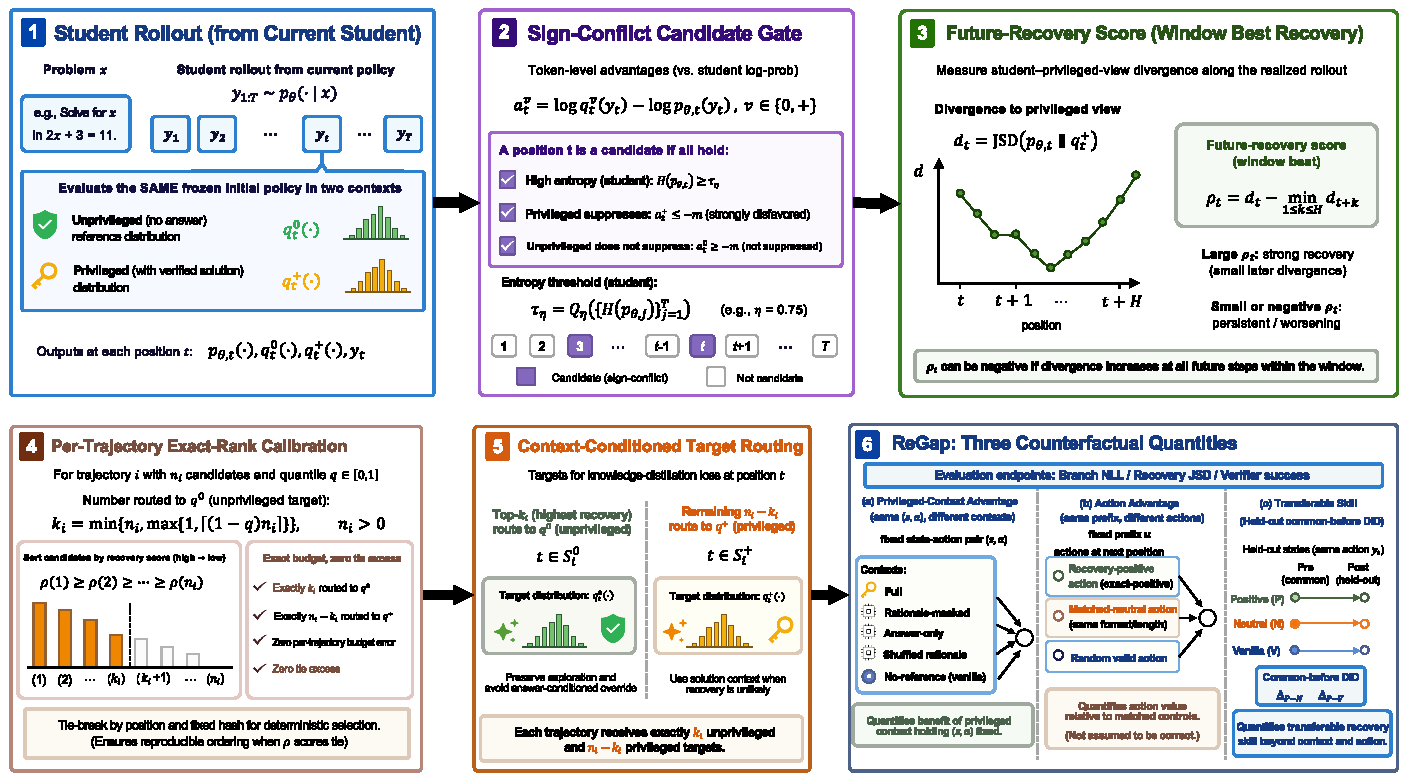
\includegraphics[width=\textwidth]{figures/rift_main_figure_ppt_outlined_cropped.pdf}
\caption{Method overview. Panels 1--5 define \RIFT{}: the current student
generates a rollout; two contextual views of the same frozen initial policy
produce $q^0$ (unprivileged, no answer) and $q^+$ (privileged, verified
solution); a sign-conflict gate identifies candidate tokens; window-best
future recovery scores their realized continuations; exact rank fixes the
per-trajectory route count; and context-conditioned routing assigns
recoverable tokens to $q^0$ and persistent tokens to $q^+$. Panel~6 defines
the three \ReGap{} quantities. Its diagrams are schematic and line positions
are not quantitative results; evaluated outcomes include branch NLL, recovery
JSD, and verifier success. We use $m=0.05$, $H=32$, $q=0.25$, and an entropy
quantile threshold $\tau_\eta$ with $\eta=0.75$. Future information and routing
are used only during training.}
\label{fig:overview}
\end{figure*}

\section{Related Work}

\subsection{Distillation on Student-Induced Distributions}

Knowledge distillation was introduced as distribution matching between a
teacher and student \citep{hinton2015distilling}, then extended to sequences,
policies, representations, same-capacity students, and iterative self-training
\citep{kim2016sequence,rusu2015policy,sun2019patient,
furlanello2018bornagain,xie2020noisystudent}. Sequential prediction adds
learner-induced state shift: early student actions determine later prefixes.
DAgger collects supervision on learner states, and GKD/MiniLLM apply this
principle to autoregressive language models
\citep{ross2011reduction,agarwal2024gkd,gu2024minillm}. OPSD uses privileged
reasoning context to supervise a student's own rollout with a frozen
self-teacher \citep{zhao2026opsd}. \RIFT{} addresses the token-level question
of which contextual view should supervise each fork.

\subsection{Controlling Privileged Reasoning Supervision}

Process supervision assigns feedback to intermediate reasoning steps rather
than only the final answer \citep{uesato2022process,lightman2023verify}. OPSD
conditions a dense teacher distribution on a verified solution, which can
alter local credit at uncertain forks \citep{kaur2026rethinking,peng2026adopsd}.
Position-aware OPD and ReNIO change where supervision is weighted
\citep{xie2026position,lin2026renio}; PHF, RLCSD, Purified OPSD, and AR-OPD
change the representation or target being distilled
\citep{li2026phf,pan2026rlcsd,shen2026purified,zhang2026aropd}; DemoPSD and
AD-OPSD use current disagreement or suppression
\citep{li2026demopsd,peng2026adopsd}; and Hindsight Self-Distillation uses a
successful peer continuation \citep{li2026hsd}. \RIFT{} instead measures
reconvergence on the realized rollout, fixes a local exact-rank budget, and
switches recoverable conflicts from $q^+$ to the unprivileged view $q^0$ while
retaining dense supervision.

\subsection{Recovery, Search, and Transfer}

STaR, Reflexion, Tree of Thoughts, and adaptive test-time compute exploit
information revealed after an initial decision
\citep{zelikman2022star,shinn2023reflexion,yao2023tree,snell2024scaling}.
\RIFT{} converts this trajectory property into a training-time routing signal.
A separate identification question remains: privileged context may rescue a
fixed branch without making its action better or transferring skill to the
no-reference student. Context-return experiments expose this distinction
\citep{wang2026context}; \ReGap{} estimates it through matched fixed-context,
fixed-prefix, and held-out transfer comparisons.

\section{RIFT: Future-Recovery Target Routing}
\label{sec:rift}

\subsection{Student Rollout and Contextual Reference Views}

Let $x$ denote a problem, $r$ a verified solution, and
$y=(y_1,\ldots,y_T)$ an on-policy student rollout. At position $t$, the
trainable student distribution is
\begin{equation}
p_{\theta,t}=p_\theta(\cdot\mid x,y_{<t}).
\end{equation}
OPSD is defined by applying one model under student and privileged contexts.
Its experimental fixed-teacher implementation holds the target at the initial
policy while the student LoRA parameters update. We adopt that implementation:
$\bar\theta=\theta_0$ denotes the frozen initial policy and $\theta$ denotes the
current student parameters. We evaluate $p_{\bar\theta}$ under two contexts.
The privileged reference distribution observes the verified solution,
\begin{equation}
q^+_t=q_{\bar\theta}(\cdot\mid x,r,y_{<t}),
\end{equation}
whereas the unprivileged reference distribution receives the inference-time
context only,
\begin{equation}
q^0_t=q_{\bar\theta}(\cdot\mid x,y_{<t}).
\end{equation}
Thus $q^+$ and $q^0$ share one frozen parameter set and differ only in
conditioning context; they are two reference views, not separate teacher
models.
Standard OPSD distills the privileged distribution densely along the rollout:
\begin{equation}
\mathcal L_{\mathrm{OPSD}}
=\frac{1}{T}\sum_{t=1}^{T}\JSD(p_{\theta,t}\Vert q^+_t).
\label{eq:opsd}
\end{equation}
The rollout is on-policy and the target is conditioned on hindsight. \RIFT{}
retains the same rollout and frozen initial policy while making its conditioning
context---privileged or unprivileged---a token-level routing decision.

\subsection{Sign-Conflict Candidate Gate}

For the sampled token $y_t$, define the privileged and unprivileged log-support
margins relative to the student:
\begin{align}
a_t^+ &= \log q_t^+(y_t)-\log p_{\theta,t}(y_t),\\
a_t^0 &= \log q_t^0(y_t)-\log p_{\theta,t}(y_t).
\end{align}
For trajectory $y_{1:T}$, define the student-entropy threshold
\begin{equation}
\tau_\eta=Q_\eta\!\left(\{H(p_{\theta,j})\}_{j=1}^{T}\right).
\end{equation}
A token is a routing candidate when the student is uncertain, the privileged
view suppresses the sampled action, and the unprivileged view does not reject
it by the same margin:
\begin{equation}
C_t=\Ind\!\left[
H(p_{\theta,t})\geq \tau_\eta
\;\land\;a_t^+\leq -m
\;\land\;a_t^0\geq -m
\right].
\label{eq:candidate}
\end{equation}
The formal recipe uses $\eta=0.75$ and suppression margin $m=0.05$.

\subsection{Future-Recovery Score on the Realized Rollout}

Let
\begin{equation}
d_t=\JSD(p_{\theta,t}\Vert q_t^+)
\end{equation}
measure current divergence from the privileged reference. For a look-ahead window
$H$, the recovery score is
\begin{equation}
\rho_t=d_t-\min_{1\leq k\leq H}d_{t+k}.
\label{eq:recovery}
\end{equation}
A large $\rho_t$ means that disagreement at $t$ falls later on the same student
continuation. A score near zero marks persistent divergence; $\rho_t<0$ means
divergence increases at every valid future position in the window. We use
$H=32$ future tokens in the primary configuration. Positions without a full
valid future window are excluded from the primary candidate set.

Equation~\ref{eq:recovery} is an observed-rollout hindsight statistic. It does
not estimate the counterfactual value of every alternative action. This
distinction motivates the separate \ReGap{} analysis below.

\subsection{Per-Trajectory Exact-Rank Calibration}

For trajectory $i$, let $\mathcal C_i$ be its candidate set and
$n_i=|\mathcal C_i|$. Given quantile parameter $q$, the prescribed route count
is
\begin{equation}
k_i=
\begin{cases}
\min\{n_i,\max\{1,\lceil(1-q)n_i\rceil\}\}, & n_i>0,\\
0, & n_i=0.
\end{cases}
\label{eq:budget}
\end{equation}
Candidates are sorted lexicographically by decreasing $\rho_t$, increasing
token position, and a fixed integer hash. The first $k_i$ receive $g_t=1$; all
others receive $g_t=0$. The primary $q=0.25$ configuration therefore selects
approximately the highest-recovery 75\% of candidates while maintaining an
exact deterministic count.

A threshold quantile instead applies
\begin{equation}
g_t=\Ind[t\in\mathcal C_i\land \rho_t\geq
Q_q(\{\rho_j:j\in\mathcal C_i\})].
\end{equation}
Quantized ties make this count data-dependent. Exact rank separates the choice
of \emph{how many} tokens to route from the values and ties of their scores.

\subsection{Context-Conditioned Target Routing}

The routed loss is
\begin{align}
\mathcal L_{\RIFT}
&=\frac{1}{T}\sum_{t=1}^{T}\Big[
(1-g_t)\JSD(p_{\theta,t}\Vert q_t^+)\nonumber\\
&\hspace{5.6em}+g_t\JSD(p_{\theta,t}\Vert q_t^0)\Big].
\label{eq:riftloss}
\end{align}
The $k_i$ highest-recovery candidates receive $g_t=1$ and target $q_t^0$;
remaining candidates and non-candidate positions receive $g_t=0$ and target
$q_t^+$. Every position therefore retains a dense distillation loss. The
unprivileged distribution acts as a stable reference rather than a trainable
self-target.

\paragraph{Training and inference cost.}
The student rollout and both contextual reference distributions are needed
during training.
Future recovery is computed after the rollout has been generated, so it does
not add inference-time look-ahead. At deployment, \RIFT{} is an ordinary
fine-tuned student with no teacher, route classifier, verifier, or future
window.

\paragraph{Implementation invariants.}
Every formal run records candidate count, target route count, actual route
count, boundary ties, per-trajectory budget error, candidate checksum, and
route-mask checksum. A formal run is accepted only if all steps are finite and
the exact-budget error is zero.

\section{ReGap: Three Counterfactual Quantities}
\label{sec:regap}

Let $s=(x,y_{<t})$ be a fixed student state, $a=y_t$ a fixed branch action,
and $c$ a problem-aligned privileged rationale. Let $V(s,a,c)$ denote a
continuation outcome such as verifier success, negative branch NLL, or negative
recovery JSD. A fixed-action rescue gap compares privileged and unprivileged
contexts:
\begin{equation}
G_{\mathrm{ctx}}(s,a)=V(s,a,c)-V(s,a,\varnothing).
\label{eq:regap}
\end{equation}
This gap measures the value of privileged context for one state--action pair.
\ReGap{} complements it with two further comparisons so that context, action,
and transfer are identified separately.

\paragraph{Privileged-context advantage.}
The state and action $(s,a)$ remain fixed while the continuation context varies
among full verified solution, rationale-masked, answer-only, shuffled-rationale,
and no-reference conditions. The resulting contrasts quantify which component
of privileged context accounts for rescue.

\paragraph{Action advantage.}
The prefix remains fixed while the next action varies among a recovery-positive
action, a matched-neutral action of the same format and length, and a random
valid action. Forced continuations from the common prefix quantify branch
action value relative to matched controls. Matching uses problem, prefix
position, original NLL/JSD, length, and difficulty.

\paragraph{Transferable skill.}
We train positive ($P$), matched-neutral ($N$), and vanilla ($V$) arms, then
evaluate the same action on problem-disjoint held-out states without privileged
context. Let $\mathrm{Pre}_A$ and $\mathrm{Post}_A$ denote the common-before and
held-out outcomes for arm $A$. The registered contrasts are
\begin{equation}
\begin{aligned}
\Delta_{P-N}&=(\mathrm{Post}_P-\mathrm{Pre}_P)
 -(\mathrm{Post}_N-\mathrm{Pre}_N),\\
\Delta_{P-V}&=(\mathrm{Post}_P-\mathrm{Pre}_P)
 -(\mathrm{Post}_V-\mathrm{Pre}_V).
\end{aligned}
\label{eq:regap_did}
\end{equation}
These three quantities support different conclusions: context advantage
measures the benefit of privileged information at fixed $(s,a)$; action
advantage measures the value of the branch itself; and the common-before
difference-in-differences measures recovery retained after privileged context
is removed. \RIFT{} uses the first quantity to arbitrate supervision while
\ReGap{} tests the other two explicitly.

\section{Experimental Setup}

\subsection{Training Protocol}

Experiments use Qwen3-4B \citep{yang2025qwen3} and a frozen 29,434-example
OpenThoughts Math 30K OPSD corpus
\citep{zhao2026opsd,guha2025openthoughts}. The student is adapted with LoRA
rank 64 and scale 128 over attention and feed-forward projections. Both
reference distributions use the same frozen initial policy and differ only in
access to the verified solution. The controlled routing study matches
optimizer steps, effective batch, data order, rollout length, and training
tokens across methods: 50 updates at learning rate $5\times10^{-6}$ with
1,024-token on-policy rollouts, temperature 1.1, top-$p$ 0.95, and top-$k$ 20.
The registered \RIFT{} configuration uses entropy quantile 0.75, sign margin
0.05, recovery window 32, and exact-rank $q=0.25$.

The horizon-confirmatory study restarts Matched OPSD and \RIFT{} from the same
initial model for seeds 42--46 and fixes checkpoint 100 as its endpoint before
evaluation; checkpoints 25/50/75 describe the learning curve without selecting
the reported endpoint. Cross-scale tests use Qwen3-1.7B and Qwen3-8B with the
same controlled budget and no router retuning. Results from different training
budgets appear in separate table blocks.

The code-domain replication trains Qwen3-4B on OpenThoughts Coding 30K
\citep{guha2025openthoughts}. Base, matched OPSD, ReNIO
\citep{lin2026renio}, and \RIFT{} share train seed 42, a fixed evaluation
seed and protocol, and checkpoint 100.

\subsection{Evaluation}

The registered comparison evaluates frozen 30-problem snapshots of AIME24,
AIME25, and HMMT February 2025
\citep{huggingfaceh4aime2024,yentinglinaime2025,matharenahmmt2025}, with 12
completions per problem. The expanded SixBench evaluation adds MATH-500,
AMC23, and HMMT November 2025, for 660 problem clusters and 7,920 completions
per checkpoint. Its primary score is the unweighted mean of the six
benchmark-level Avg@12 values; the micro average is secondary because
MATH-500 contributes 500 of 660 problems. A frozen \texttt{math-verify}
v0.8.0 evaluator \citep{kydlicek2024mathverify} scores the final balanced
\verb|\boxed{...}| expression. Decoding parameters, dataset hashes, and exact
record counts are fixed across methods and listed in the supplement.

For code, HumanEval+ and MBPP+ are evaluated with EvalPlus v0.3.1
\citep{liu2023evalplus}, using four completions per problem. Code Macro is the
unweighted mean of the two benchmark-level Avg@4 scores.

\subsection{Baselines and Controls}

The controlled comparison includes matched OPSD, three exact-budget random
masks, Current-JSD routing, a zero-loss target ablation, AD-OPSD
\citep{peng2026adopsd}, and DemoPSD \citep{li2026demopsd}. Signal analysis
compares entropy, position, current JSD, sampled-token suppression margin, AD
risk, past recovery, shuffled future, true future recovery, and current
covariates with or without future recovery. The external panel includes
a zero-update Base model, 100-update SFT and GRPO training-paradigm baselines,
and paper-faithful PHF and Purified OPSD reproductions. All rows use the same
frozen SixBench evaluator; trained Qwen3-4B rows are evaluated at update 100.

\subsection{Signal and Counterfactual Data}

The forced-continuation study contains 512 candidate branches from 128
problems, with four fixed continuation seeds per branch (2,048 continuations).
The robust-recovery label has 442 positives among 512 candidates (86.33\%).
Predictors are evaluated out of fold. Precision@25\% uses equal selection
coverage, and uncertainty is clustered by problem.

The \ReGap{} transfer study uses three training seeds. Each seed contains 24
complete records from the same 17 problem clusters, evaluated under
exact-positive, matched-neutral, and vanilla exposures. Balance checks attain a
maximum absolute standardized mean difference of 0.02385, and each replay arm
exposes 10\% of eligible tokens.

\subsection{Statistical Reporting and Provenance}

Problems, rather than individual stochastic completions, are the unit of
inference. Seed-specific intervals resample problem clusters; pooled analyses
hierarchically resample seed and benchmark/problem. Primary comparisons use
two-sided cluster-aware tests and Holm correction where applicable. The
supplement reports evaluator and data versions, seeds, benchmark numerators,
record counts, identifiers, and resampling protocols; every comparison is
computed from one frozen result snapshot.

For the code-domain replication, \RIFT{}--Matched OPSD is the sole
prespecified primary contrast and is reported without multiplicity adjustment.
The three secondary contrasts form a separate Holm-corrected family.

\section{Results}

\subsection{Controlled Budget-Matched Performance}

The registered controlled comparison gives consistent gains. At seed 42,
\RIFT{} obtains 689/1,080 (63.80), compared with 678/1,080 (62.78)
for matched OPSD, a gain of 1.02 points. At seed 43, \RIFT{} obtains 673/1,080
(62.31), compared with 654/1,080 (60.56), a gain of 1.76 points. The two-seed
mean is 63.06 versus 61.67; the 1.39-point gain has a hierarchical 95\%
interval of [0.23, 2.55]. A registered seed-44 comparison yields 676/1,080
(62.59) for \RIFT{} and 650/1,080 (60.19) for matched OPSD, a 2.41-point
gain. Under this common training and evaluation budget, \RIFT{} has the
highest displayed Avg@12 point estimate among the evaluated methods.

Current-JSD routing obtains 60.19, compared with 61.76 for the three-mask
random-routing aggregate. The paired Current-JSD--random interval is
[-3.20, 0.09] ($p=0.0718$), indicating that immediate disagreement magnitude
does not account for the controlled \RIFT{} result.

\subsection{Training-Horizon, Benchmark, and Scale Robustness}

Table~\ref{tab:confirmatory} fixes one SixBench evaluator and keeps training
budgets separate. At the controlled 50-update budget, the pooled 4B comparison
improves over Matched OPSD by $+1.69$ Macro points and improves all six
benchmarks.
\WOneResultSentence{} \ScaleResultSentence{}

\begin{table*}[t]
\centering
\small
\setlength{\tabcolsep}{1.5pt}
\textit{Panel A: Qwen3-4B training-paradigm and strong-baseline leaderboard}\par
\begin{tabular*}{\textwidth}{@{\extracolsep{\fill}}lrrrrrrrr@{}}
\toprule
Method & Updates & A24 & A25 & M500 & AMC23 & H-Feb & H-Nov & Macro \\
\midrule
Base & 0 & \BaseAIMEFour & \BaseAIMEFive & \BaseMATH & \BaseAMC & \BaseHFeb & \BaseHNov & \BaseHundred \\
SFT & 100 & \SFTAIMEFour & \SFTAIMEFive & \SFTMATH & \SFTAMC & \SFTHFeb & \SFTHNov & \SFTHundred \\
GRPO & 100 & \GRPOAIMEFour & \GRPOAIMEFive & \GRPOMATH & \GRPOAMC & \GRPOHFeb & \GRPOHNov & \GRPOHundred \\
\midrule
Matched OPSD & 100 & \WOneMatchedAIMEFour & \WOneMatchedAIMEFive & \WOneMatchedMATH & \WOneMatchedAMC & \WOneMatchedHFeb & \WOneMatchedHNov & \WOneMatchedPooled \\
PHF & 100 & \PHFAIMEFour & \PHFAIMEFive & \PHFMATH & \PHFAMC & \PHFHFeb & \PHFHNov & \PHFHundred \\
Purified OPSD & 100 & \PurifiedAIMEFour & \PurifiedAIMEFive & \PurifiedMATH & \PurifiedAMC & \PurifiedHFeb & \PurifiedHNov & \PurifiedHundred \\
\best{\RIFT{} (ours)} & 100 & \best{\WOneRiftAIMEFour} & \best{\WOneRiftAIMEFive} & \best{\WOneRiftMATH} & \best{\WOneRiftAMC} & \best{\WOneRiftHFeb} & \best{\WOneRiftHNov} & \best{\WOneRiftPooled} \\
\bottomrule
\end{tabular*}
\textit{Panel B: Qwen3 matched model-scale checks at 50 updates}\par
\begin{tabular*}{\textwidth}{@{\extracolsep{\fill}}llrrrrrrr@{}}
\toprule
Model & Method & A24 & A25 & M500 & AMC23 & H-Feb & H-Nov & Macro \\
\midrule
1.7B & Matched OPSD & \ScaleOneSevenMatchedScores & \ScaleOneSevenMatched \\
1.7B & \best{\RIFT{} (ours)} & \ScaleOneSevenRiftScores & \best{\ScaleOneSevenRift} \\
\midrule
4B & Matched OPSD & \ScaleFourMatchedScores & \ScaleFourMatched \\
4B & \best{\RIFT{} (ours)} & \ScaleFourRiftScores & \best{\ScaleFourRift} \\
\midrule
8B & Matched OPSD & \ScaleEightMatchedScores & \ScaleEightMatched \\
8B & \best{\RIFT{} (ours)} & \ScaleEightRiftScores & \best{\ScaleEightRift} \\
\bottomrule
\end{tabular*}
\caption{SixBench Avg@12 scores under one frozen evaluator. A24/A25, M500, H-Feb, and H-Nov denote
AIME24, AIME25, MATH-500, HMMT-Feb, and HMMT-Nov. Macro is the unweighted mean
of all six columns. Base uses the initial model without training; all other
Panel-A rows use 100 updates. \RIFT{}$-$Matched Macro gains are $+2.15$, $+1.76$,
$+1.69$, and $+2.13$ points for 4B/100, 1.7B/50, 4B/50, and 8B/50.}
\label{tab:confirmatory}
\end{table*}

\BaselineResultSentence{}

\paragraph{Code-domain replication.}
At checkpoint 100, \RIFT{} reaches 86.95 HumanEval+, 78.02 MBPP+, and 82.49
Code Macro, versus 81.89 Macro for matched OPSD. The sole prespecified primary
contrast is \CodeRiftVsMatchedDelta{} points (95\% problem-cluster CI
\CodeRiftVsMatchedCI{}, raw $p=\CodeRiftVsMatchedRawP$). The
\CodeRiftVsReNIODelta{}-point secondary contrast over ReNIO does not reject
after Holm correction ($p=\CodeRiftVsReNIOHolmP$); complete benchmark and
multiplicity tables are in the supplement.

\subsection{What Does Future Recovery Predict?}

Figure~\ref{fig:routing}(a) summarizes signal validity. Future recovery alone
reaches AUPRC 0.90980, a positive but non-significant increment
of 0.00331 over current covariates alone (95\% CI [-0.0012, 0.0078],
$p=0.149$). Combining future recovery with current covariates reaches AUPRC
0.91840 and improves over current covariates by 0.01191 (95\% CI
[0.0049, 0.0188], $p=0.0018$). The AUROC analysis shows the same pattern:
future recovery alone changes AUROC by 0.00249 ($p=0.42$), whereas the combined
predictor improves AUROC by 0.00689 (95\% CI [0.0015, 0.0123], $p=0.013$).
Future recovery contributes statistically detectable information in the joint
router, while the future-only model provides a smaller standalone increment.
This complementarity is the intended use of recovery: current features
describe the fork itself, whereas future recovery summarizes whether its
disagreement contracts along the realized continuation.

The positive prevalence is 86.33\%, so the prevalence-matched random AUPRC
baseline is approximately 0.8633. Relative to this baseline, current-only,
future-only, and future-plus-current yield absolute AP lifts of
0.0432/0.0465/0.0551 and normalized AP values of 0.316/0.340/0.403,
respectively. Future-only therefore adds a small standalone increment, whereas
the combined predictor supplies the strongest prevalence-adjusted
discrimination. AUROC is reported alongside AP to remain insensitive to the
class prior. When persistent branches (70/512) are positive, true future
improves over current-only by \FuturePersistentAUPRCDelta{} AUPRC
(95\% CI \FuturePersistentAUPRCCI{}, Holm $p=\FuturePersistentAUPRCP$)
and \FuturePersistentAUROCDelta{} AUROC (95\% CI
\FuturePersistentAUROCCI{}, Holm $p=\FuturePersistentAUROCP$).
Future plus current is strongest on persistent AUPRC/AUROC
(\FutureCurrentPersistentAUPRC{}/\FutureCurrentPersistentAUROC{}) and on
balanced accuracy, MCC, Brier, and ECE; full prevalence-aware diagnostics
appear in the supplement.

The downstream score ablation holds the candidate gate, token partition,
exact-rank budget, and target mapping fixed. True-future routing improves over
current-only, shuffled future does not, and future plus current gives the
largest gain (Table~\ref{tab:downstream-score}).
Because route count and target mapping remain fixed across rows, this comparison
isolates candidate ordering rather than supervision volume or loss source.

\begin{table}[t]
\centering
\small
\setlength{\tabcolsep}{1.5pt}
\begin{tabular}{@{}lrrr@{}}
\toprule
Score & Macro & $\Delta$ [95\% CI] & Holm $p$ \\
\midrule
Current-only & \CurrentOnlyDownstream & -- & -- \\
Future-shuffled & \ShuffledDownstream & \ShuffledVsCurrentDelta{} \ShuffledVsCurrentCI & \ShuffledVsCurrentP \\
True future & \best{\TrueFutureDownstream} & \best{\FutureVsCurrentDelta{} \FutureVsCurrentCI} & \best{\FutureVsCurrentP} \\
Future + current & \best{\FutureCurrentDownstream} & \best{\FutureCurrentVsCurrentDelta{} \FutureCurrentVsCurrentCI} & \best{\FutureCurrentVsCurrentP} \\
\bottomrule
\end{tabular}
\caption{Downstream routing-score ablation under a fixed candidate gate,
exact-rank $q25$ budget, token partition, and target map. Differences are
relative to Current-only.}
\label{tab:downstream-score}
\end{table}

\begin{figure*}[t]
\centering
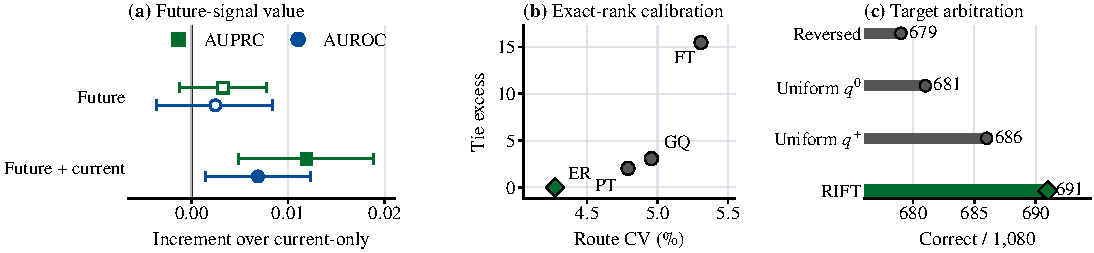
\includegraphics[width=\textwidth]{figures/rift_routing_diagnostics.pdf}
\caption{Routing diagnostics. (a) Problem-cluster 95\% intervals for the
increment over current-only prediction; filled markers exclude zero.
(b) Calibration rules plotted by route-fraction CV and tie excess, where
lower-left is better. Exact rank attains the lowest CV and zero tie excess.
FT, GQ, PT, and ER denote fixed threshold, global $q25$, per-trajectory
threshold, and exact-rank $q25$.
(c) Correct counts for context-conditioned target policies under the same
token partition and training budget.}
\label{fig:routing}
\end{figure*}

\subsection{Exact Rank Controls the Local Budget}

Exact-rank routing is the only evaluated calibration rule with zero tie excess
and exact local count by construction. It also has the lowest displayed
route-fraction coefficient of variation, 0.04276, compared with 0.04791 for a
per-trajectory threshold and 0.05308 for a fixed threshold. It makes the
intervention count reproducible under quantized scores
and isolates routing quality from accidental budget changes. The complete
calibration table is in the supplement; Figure~\ref{fig:routing}(b) visualizes
the joint calibration tradeoff.

\subsection{Context-Conditioned Target Arbitration}

With the token partition fixed, recoverable $\to q^0$ and persistent $\to q^+$
scores 691/1,080. Uniform $q^0$, uniform $q^+$, and the reversed assignment
score 681, 686, and 679, respectively (Figure~\ref{fig:routing}c). The proposed
direction therefore gains 0.93, 0.46, and 1.11 percentage points over the
three controls under the same partition and training budget. The paired
intervals for Proposed--Uniform $q^0$, Proposed--Uniform $q^+$, and
Proposed--Reversed are \ArbVsQZeroCI{}, \ArbVsQPlusCI{}, and
\ArbVsReversedCI{}, with Holm-adjusted $p$ values $\ArbVsQZeroP$,
$\ArbVsQPlusP$, and~$\ArbVsReversedP$, respectively.
\ArbitrationResultSentence{}

\subsection{ReGap Separates Recovery Transfer from Matched Controls}

Across three seeds, positive exposure lowers Branch NLL versus matched neutral
by $1.361\times10^{-4}$ (95\% CI
$[1.439\times10^{-5},2.632\times10^{-4}]$, $p=0.0285$) and recovery JSD by
$2.242\times10^{-5}$ (95\% CI
$[1.323\times10^{-5},3.221\times10^{-5}]$, $p<0.0001$). Recovery JSD also
improves versus vanilla; Branch NLL has the intended direction but does not
exclude zero. Thus three of four registered pooled contrasts pass
and the full interval table is in the supplement.

\section{Discussion}

Figure~\ref{fig:overview} separates three roles: future recovery orders
candidates, exact rank fixes the local allocation, and target arbitration
selects the contextual view supplying each loss. Together they connect the
temporal signal to its intervention count and target direction. The registered
triad, SixBench, cross-scale, and code-domain results extend the positive effect
across training horizons, model sizes, and program synthesis.

\ReGap{} clarifies whether privileged improvement belongs to context, the
branch action, or transferable student skill. Across three seeds, positive
exposure separates from matched neutral on both endpoints and from vanilla on
recovery JSD; only Branch NLL versus vanilla retains an interval containing
zero. Thus \ReGap{} interprets recovery-informed routing rather than adding a
training reward.

\subsection{Closing the Mechanism--Performance Chain}

The ablations close three links. With gate, budget, partition, and target map
fixed, true future improves the router, shuffled future does not, and future
plus current is strongest (Table~\ref{tab:downstream-score}). Exact rank removes
tie excess and minimizes route-fraction variation. Under the same partition,
recoverable $\to q^0$ and persistent $\to q^+$ beats both uniform targets and
the reversed assignment in all three Holm-adjusted tests. \RIFT{} also leads
the displayed checkpoint-100 baselines and retains positive Macro gains at
1.7B, 4B, and 8B.

This decomposition also gives an operational interpretation of the method. The
candidate gate identifies disagreements that may warrant intervention; future
recovery orders those positions by the student's realized ability to
reconverge; exact rank converts that ordering into a deterministic local
allocation; and target arbitration selects the contextual view that supplies
supervision. These components are used only during training. At inference,
\RIFT{} deploys the student alone, so the privileged solution, recovery window,
and routing computation add no serving-time overhead. The separation further
attributes failures to candidate detection, score ordering, budget allocation,
or target direction.

\section{Limitations}

Future recovery depends on window length, rollout stochasticity, and sequence
censoring; $q=0.25$, $H=32$, and the candidate thresholds define one operating
point. The main study uses mathematical training data, Qwen3-family models, and
a 660-problem SixBench evaluation. The code-domain replication broadens the
task family but uses one Qwen3-4B training seed; its intervals capture
problem-cluster and generation uncertainty, not training-seed variation.
Non-4B scale checks likewise use one training seed. The 86.33\% recovery
prevalence motivates persistent-class and prevalence-adjusted metrics.
SixBench strong-baseline and cross-scale rows are point-estimate checks, while
the registered comparison supplies inferential analysis. Three of four pooled
\ReGap{} contrasts exclude zero; Branch NLL versus vanilla is less precisely
estimated.

\section{Conclusion}

\RIFT{} combines future reconvergence with exact-rank supervision. It improves
matched OPSD by 1.39 points in the registered Qwen3-4B comparison (95\% CI
[0.23, 2.55]), by 2.15 SixBench Macro points at checkpoint 100, and by
\CodeRiftVsMatchedDelta{} Code Macro points (95\% CI
\CodeRiftVsMatchedCI{}) in the code replication. \ReGap{} separates context,
action, and transferable-skill effects, completing a framework for deciding
when a student should trust privileged context.

\bibliography{RIFT_AAAI27_refs}

\end{document}
